\documentclass[a4paper,11pt]{article}
\usepackage[T1]{fontenc}
\usepackage[francais]{babel}
\usepackage[utf8x]{inputenc}
\usepackage{lmodern}
\usepackage{apacite}
\usepackage{fourier}
\usepackage{graphicx}


\title{La pratique réflexive dans la formation des enseignants de l'école normale aux ESPE}
\author{Sylvain Golder}

\begin{document}

\maketitle
%\tableofcontents

\begin{quote}
  Mais entre l'art ainsi défini et la science proprement dite, il y a place pour une attitude mentale intermédiaire. Au lieu d'agir sur les choses ou sur les êtres suivant des modes déterminés, on réfléchit sur les procédés d'action qui sont ainsi employés, en vue non de les connaître et de les expliquer", mais d'apprécier ce qu'ils valent, s'ils sont ce qu'ils doivent être, s'il n'est pas utile de les modifier et de quelle manière, voire même de les remplacer totalement par des procédés nouveaux. Ces réflexions prennent la forme de théories ; ce sont des combinaisons d'idées, non des combinaisons d'actes, et, par là, elles se rapprochent de la science. Mais les idées qui sont ainsi combinées ont pour objet, non d'exprimer la nature de choses données, mais de diriger l'action. Elles ne sont pas des mouvements, mais sont toutes proches du mouvement, qu'elles ont pour fonction d'orienter. Si ce ne sont pas des actions, ce sont, du moins, des programmes d'action, et par là elles se rapprochent de l'art. Telles sont les théories médicales, politiques, stratégiques, etc. Pour exprimer le caractère mixte de ces sortes de spéculations, nous proposons de les appeler des théories pratiques. La pédagogie est une théorie pratique de ce genre. Elle n'étudie pas scientifiquement les systèmes d'éducation, mais elle y réfléchit en vue de fournir à l'activité de l'éducateur des idées qui le dirigent.  \cite{durkheim11}
\end{quote}

\part*{Introduction}
Pour Émile Durkheim \cite{durkheim11}, la pédagogie est une \emph{théorie-pratique} c'est à dire une réflexion vers l'action, ce qui fait dire à Michel Fabre \cite{fabre02} que \emph{la science est de l'ordre du savoir comprendre ou expliquer, l'art relève du savoir faire et la pédagogie du savoir sur le faire qui est en même temps un savoir pour faire}. Ainsi la pédagogie est nécessairement réflexive, l'action pédagogique ne peut exister sans réflexion sur elle même. Ce statut praxéologique implique une formation adéquate des acteurs de l'éducation, notamment des enseignants. Or il nous a semblé pertinent d'analyser ce que pouvait être une formation professionnelle historiquement parlant pour replacer le processus de la mastérisation dans le temps long, qui est celui qui accompagne la réflexion, constante, de la formation des enseignants de la république depuis – au moins – la naissance des écoles normales. A la suite de John Dewey, nous pouvons dire que la pensée nait de l'expérience, que c'est l'expérience qui forme la pensée ainsi que le note Gérard Deledalle \cite{deledalle65} : \emph{dès qu'il y a rupture de continuité entre l'activité et l'objet de l'activité, quand, dans le cours de l'expérience, nous rencontrons un obstacle, commence la réflexion qui permet de rétablir la continuité}. \\

Pour l'enseignant la pratique réflexive est nécessaire puisqu'il est en contact avec l'imprévisible, les enfants ne peuvent être agis, l'apprentissage découle des interrelations entre l'enseignant et les apprenants, de plus il se doit de se tenir au courant des avancées de la recherche et emprunter aux savoirs scientifiques ainsi le bulletin officiel de l'éducation nationale n°1 du 4 janvier 2007 stipule qu'en \emph{formation professionnelle initiale, les maîtres doivent être initiés à la recherche scientifique, à ses résultats et à ses applications dans l'enseignement. Les pratiques didactiques et pédagogiques doivent se nourrir de l'évolution des connaissances.} Depuis la mise en place des instituts universitaires de formation des maîtres (IUFM) en 1990, les futurs professeurs des écoles doivent produire un mémoire professionnel en deuxième année de formation. Ce mémoire est le lieu privilégié, mais non unique, de la réflexivité enseignante lors de la formation initiale. Il est également le lieu privilégié de la diplomatie entre l'école professionnelle et l'université. Sans donner à l'université l'exclusivité de la recherche\footnote{De nombreux pédagogues mènent des recherches avec ou sans l'université que ce soit au laboratoire de recherche coopérative de l'ICEM, aux cahiers pédagogiques ou bien de manière plus isolée.}, le rapprochement de ces deux mondes est un choix qui permet en théorie de rapprocher théorie et pratique, recherche et formation. 
\\

Ainsi nous tâcherons de montrer la permanence historique d'un projet professionnalisant et réflexif dans la formation des enseignants puis nous aborderons la question de l'écart entre le prescrit et le réel avant de nous demander en quoi l'injonction réflexive est opérante pour la formation initiale des IUFM puis des ESPE.


\part{La permanence d'un projet professionnalisant dans la formation des enseignants}

Dès lors qu'une formation des enseignants du primaire est conçue, se pose la question de la professionnalisation des enseignements et de la pédagogie. Je distingue ici volontairement primaire et secondaire car les formations et les concours du secondaire (notamment l'agrégation) sont davantage disciplinaires et moins pédagogiques. Le certificat d'aptitude pédagogique, créé en 1881 par l'article 3 du décret du 4 janvier, prévoit trois épreuves : une épreuve écrite, une épreuve pratique qui consiste à faire la classe et une épreuve orale de pédagogie.    

	\section{Tensions entre professionnalisation et disciplines}

Nous pouvons distinguer deux voies pour former les enseignants; la première consiste à considérer qu'il est important de maîtriser le savoir et que c'est le rapport du maître au savoir qui va être le liant de la transmission. Le triangle pédagogique de Houssaye nous indique que nous sommes alors dans le paradigme de l'enseigner de la didactique \cite{houssaye00}. La seconde considère que ce qui est déterminant, c'est avant tout la capacité de l'enseignant à faire la classe, à maintenir l'ordre et à se faire écouter des élèves. La première voie est celle qui a été privilégiée pour la formation des professeurs du secondaire, le CAPES comme l'agrégation sont des concours avant tout disciplinaires qui demandent un savoir exigeant et quasi-expert de la discipline. La seconde voie est celle qui a été privilégiée pour la formation des enseignants du primaire. Nous pouvons supposer qu'il y a là une vision de l'institution sur l'enseignement au primaire qui est général donc non exigeant et qui finalement peut-être donné par tout le monde. La loi Guizot du 21 juin 1833 ne dit pas autre chose quand elle déclare dans l'article 4 que :
\begin{quote}
\emph{Tout individu âgé de 18 ans accomplis pour exercer la profession d'instituteur primaire, et diriger tout établissement quelconque d'instruction primaire, sans autre condition que de présenter préalablement au maire de la commune où il voudra tenir école : (1) un brevet de capacité obtenu, après examen, selon le degré de l'école qu'il veut établir; (2) Un certificat constatant que l'impétrant est digne par sa moralité de se livrer à l'enseignement. Le certificat sera délivré, sur l'attestation de trois conseillers municipaux, par le maire de la commune, ou de chacune des communes où il aura résidé pendant trois ans.}
\end{quote}
La formation des instituteurs est donc pensée comme nécessairement professionnalisante, il ne s'agit pas tant d'apprendre des savoirs académiques que de savoir faire une leçon, tenir une classe et être homme de morale. Pourtant l'instituteur de la troisième république est souvent l'intellectuel du village. En effet, entre 1886 et 1914 la moyenne de baccalauréats délivrés est d'environ 7144 par an sur une population d'environ 40 millions d'individus\footnote{Contre environ 28000 en 1940, 197000 en 1974 et plus de 589000 en 2013 selon la note d'information n°6 de Mars 2014 des résultats définitifs de la session 2013 du baccalauréat.} \cite{chesnais75}. De son côté le certificat d'études primaires est délivré à environ 30\% des élèves vers 1900 et jusqu'à 50\% en 1936 \cite{lang11}. 

			\subsection{La figure de l'instituteur}
				L'instituteur est donc une figure institutionnelle, urbaine et intellectuelle dans le village d'une France massivement rurale\footnote{Selon le recensement de 1901, 45\% de la population active travaille dans les secteurs de la pêche, forêts et agriculture, 44\% en 1906 et 39\% en 1921.} Il est d'ailleurs demandé, pour les expositions universelles de 1889 et de 1900 dans les instructions générales du 31 juillet 1887 et du 29 décembre 1998, aux enseignants de rédiger une monographie sur la commune où ils exercent, ce qui constitue un travail de recherche sur l'histoire et la géographie locale, l'urbanisme, l'économie, l'agriculture, la faune et la flore etc.   
			\subsection{La réflexion pratique des enseignants}
			Mais si cette œuvre de pensée semble bien éloignée de la salle de classe, qu'en est-il de la réflexion plus pratique et donc pédagogique ? Le premier arrêté du 10 février 1837 et surtout l'arrêté du 5 juin 1880 mettent en place le système des conférences pédagogiques qui a toujours plus ou moins cours dans les actuels écoles supérieures du professorat et de l'éducation (ESPE). Ces conférences traitent de \emph{matières de pédagogie théorique et pratique} et la présence est obligatoire pour les \emph{instituteurs et institutrices publics titulaires; elle l'est aussi pour les instituteurs adjoints}. Ces conférences ont pour but de \emph{permettre à tous les instituteurs de participer à des études communes}\footnote{circulaire du 10 août 1880}.
			Cependant, même si rapidement les élèves de l'école normale vont participer aux conférences pédagogiques, nous pouvons nous demander ce qu'il en est de la formation initiale des instituteurs. 
			\subsection{Et la formation initiale ?}
			A travers les programmes d'enseignement et le programme des concours, nous allons pouvoir mettre en perspective les travaux de réflexion pédagogique des élèves-maîtres puis des futurs professeurs des écoles. En 1887, le certificat d'aptitude pédagogique comporte dans son épreuve pratique une rédaction pédagogique avec des sujets tels que : \emph{Dans quelle mesure la discipline concourt-elle à l'œuvre de l'éducation générale} \cite{cha87}. Nous pouvons voir dans les cours de Gaston Daubigny, élève-maître à l'école normale de Beauvais qu'ils mélangent des leçons de morale et d'instruction civique, avec des notions philosophiques comme \emph{l'intuition}, des méthodes de lecture et d'écriture, d'arithmétique, et à chaque fois, une liste d'ouvrages à consulter et une argumentation de trois paragraphes sur un sujet. Par exemple : \emph{Pour faire un bon instituteur il faut trois choses : un peu de savoir, du bon sens et beaucoup de discernement} \cite{dob1899}. 
			\begin{figure}[!h]
			\centering
			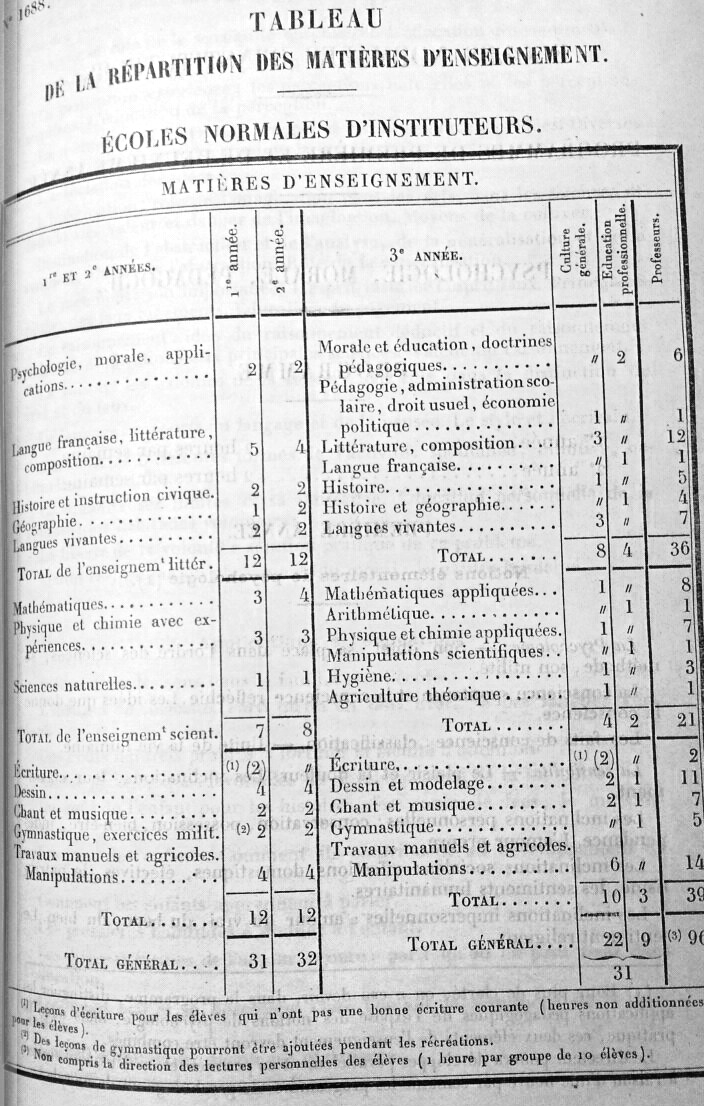
\includegraphics[width=0.6\textwidth]{prog1905.png}\\
			\caption{Le programme des matières d'enseignement de l'école normale d'instituteurs. Arrêté du 5 août 1904}
			\label{fig. 1}
			\end{figure}

			Plus tard, le programme successif instauré par la réforme de 1905 (voir fig. \ref{fig. 1}, page \pageref{fig. 1} ) marque la troisième année de l'école normale d'une empreinte résolument professionnalisante en accumulant les cours de morale, de pédagogie et les stages pratiques.
			
\section{En quête d'une identité professionnelle}
Du hussard noir de la république au professeur des écoles, la réalité du métier de l'enseignant a considérablement changé. D'abord parce que la société a elle même changé, mais avant tout parce que les élèves ont changé. En effet, si aujourd'hui l'enseignement primaire peut être considéré comme propédeutique au secondaire, le trajet suivi par les élèves de la fin du $XIX^{ème}$ siècle jusqu'au milieu du $XX^{ème}$ siècle est fondamentalement distinct, il n'y a pas à proprement parler de cohérence de ce qu'on appelle aujourd'hui un système éducatif mais plutôt des établissements différents fonctionnant selon des logiques propres. Les enfants des classes populaires fréquentent les écoles primaires gratuites jusqu'à 12 ans puis 14 ans, tandis que les enfants des classes supérieures fréquentent les établissements secondaires.  
			
			\subsection{Primaire et secondaire, une guerre... civile ?}
			Les instituteurs sont eux mêmes souvent sortis des écoles primaires supérieures et des cours complémentaires qui préparent au brevet élémentaire nécessaire à l'entrée en école normale, ils constituent donc ce qu'il convient d'appeler une élite populaire ou républicaine. Les professeurs du secondaire, pour beaucoup des agrégés\footnote{52\% des professeurs de lycée en 1898 selon Antoine Prost cité par Yves Verneuil \cite{ver04}}, et les instituteurs ne forment pas le corps et n'exercent pas encore la même profession, ce clivage marquera durablement le système scolaire français\footnote{Peut être même encore aujoud'hui lorsqu'on aperçoit parfois certaines difficultés à travailler ensemble}. Toutefois la deuxième moitié du $XX^{ème}$ siècle verra les deux ordres se fondre en degrés avec une succession progressive du primaire (le 1er degré) et du secondaire (le second degré) avec la naissance du collège unique en 1975 et la loi d'orientation de 1989 et ses fameux \emph{80\% d'une classe d'âge au bac}, chiffre symbolique quasiment atteint en 2012 (avec 77,5\% d'une classe d'âge). C'est également à la rentrée 1990 que naissent les instituts universitaires de formation des maîtres (IUFM) qui marquent un tournant dans la professionalisation des enseignants, évolution confirmée depuis avec leur intégration dans les universités en 2005 puis avec la création des écoles supérieures du professorat et de l'éducation (ESPE) en 2013.
			
			\subsection{La création des IUFM}
			La loi d'orientation de 1989, dite loi \emph{Jospin} indique la création des IUFM dans son article 17 : \emph{Sera créé, dans chaque académie, à partir du 1er septembre 1990, un institut universitaire de formation des maîtres, rattaché à une ou plusieurs universités de l'académie}. Rattachés aux universités, les IUFM doivent fournir une formation qui se veut d'emblée professionnelle, ouverte désormais à partir de la licence tout en visant à rapprocher les statuts des nouveaux professeurs des écoles et des professeurs du secondaires, certifiés, en alignant les grilles de salaires, les diplômes et les statuts\footnote{ceci sans compter le corps des agrégés, qui conserve sont statut spécifique}. Nous pouvons observer que le programme de l'IUFM dans sa version originale (1990-2010) ressemble dans sa philosophie à celui de 1905 : Successif avec une année générale d'enseignement (contre deux en 1905) et une année avec stage et mémoire. Les enseignements sont assez proches :  psychologie, morale, langue française et littérature, histoire, géographie et instruction civique, mathématiques, physique et chimie, sciences naturelles, écriture, dessin, chant et musique, gymnastique, exercices militaires, travaux manuels et agricoles lors des deux premières années d'enseignement de l'école normale en 1905 (voire figure \ref{fig. 1}, page \pageref{fig. 1}) contre du français, des mathématiques, des sciences et de la technologie, de l'histoire-géographie, des arts visuels, de l'éducation musicale, de la littérature de jeunesse, des langue vivantes étrangères ou encore de l'EPS; le tout sanctionné par le concours en fin d'année, afin de garantir que les élèves et étudiants ne souffrent pas de la présence du concours et se consacrent entièrement à leur future entrée dans le métier. Il ne s'agit pas de faire d'anachronisme en disant que les programmes sont les mêmes et que le programme de 2005 (voir figure \ref{fig. 2}, page \pageref{fig. 2}) serait une copie de celui de 1905\footnote{et ce serait oublier l'introduction des mathématiques modernes et du tiers-temps pédagogique, des querelles sur les méthodes de lectures, des progrès en psychologie du développement et des apprentissages, de la démocratisation scolaire, du relèvement du niveau du diplôme des enseignants etc.} mais pour terminer l'analogie, la deuxième année dite PE2 en 2005 et la troisième année de l'école normale en 1905 sont toutes deux marquées par la forte présence des stages et celle d'un mémoire soutenu à l'oral à la fin de l'année\footnote{mémoire qui n'a ni la même fonction, ni le même poids cependant.}.
			  \begin{figure}[!h]
			    \centering
			    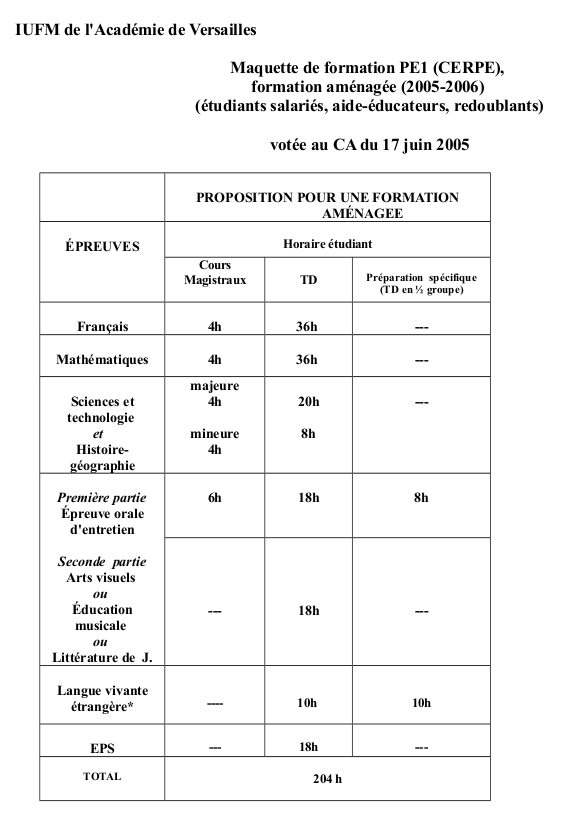
\includegraphics[width=0.6\textwidth]{prog2005.png}\\
			    \caption{Maquette de formation PE1 (CERPE), formation aménagée (2005-2006) (étudiants salariés, aide-éducateurs, redoublants)}
			    \label{fig. 2}
			  \end{figure}
			  
			  \begin{figure}[!h]
			    \centering
			    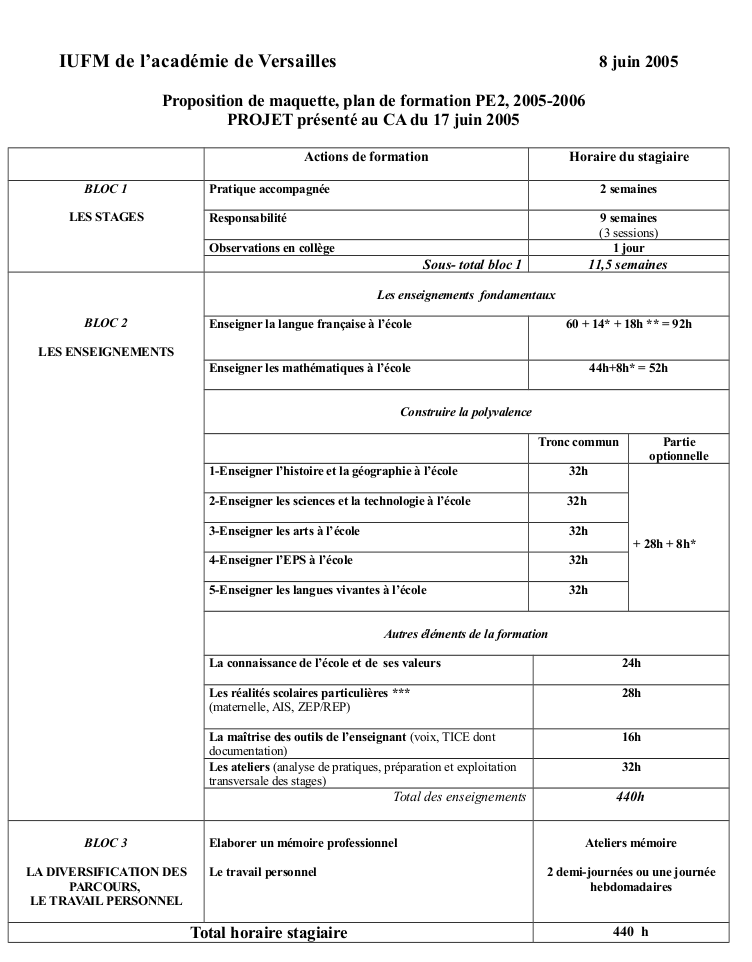
\includegraphics[width=0.6\textwidth]{prog05PE2.png}\\
			    \caption{Maquette de formation PE1 (CERPE), formation aménagée (2005-2006) (étudiants salariés, aide-éducateurs, redoublants)}
			    \label{fig. 3}
			  \end{figure}
			
			\subsection{La figure du praticien réflexif}
			L'ouvrage de Donald Schön paru en 1984 (1993 pour la traduction française) sur le concept de \emph{think in action} maladroitement traduit par \emph{savoir caché dans l'agir professionnel} marque une étape dans la théorisation du concept de reflexivité intimement lié à la profession enseignante \cite{sch93}. L'identité professionnelle de l'enseignant, en constante mutation, peut en effet se fonder sur la reflexivité comme marqueur de ce qu'est le métier enseignant, ni une théorie pure de l'éducation sans élèves, ni une pratique pure sans réflexion; une praxis ou comme l'appelait déjà Durkheim : une \emph{théorie pratique}\footnote{op. cit.}. Il nous semble que les revues éditées par les enseignants, les syndicats ou les instituts pédagogiques, aujourd'hui les blogs et les forums, les conférences pédagogiques, le rapprochement constant (et parfois contesté) d'avec l'université et les chercheurs, la recherche-action mais également la formation initiale et notamment le mémoire professionnel participent grandement de cette réflexivité des enseignants. Fondamentalement, le professeur est un praticien réflexif. 
			
\section{Faire la classe, penser la classe}
Faire la classe c'est le coeur de l'enseignement, quelque soit sa pédagogie et sa façon d'apréhender le métier, c'est de se retrouver devant ses élèves pour leur permettre d'entammer un processus d'apprentissage. Loin d'être évident, il s'agit d'utiliser ce que l'on sait (ou ce que l'on se représente) du métier, des élèves, des fonctions cognitives des enfants etc. d'une manière personnelle et réfléchie, en action. Cet acte éducatif met donc en action des savoirs, savoirs \emph{cachés} que la réflexion, la \emph{prise de conscience} ou \emph{explicitation} selon le terme de Vermersch \cite{ver94} permettent d'apprendre à connaître ses pratiques et ses compétences mais aussi, le cas échéant, de les modifier. Historiquement, la formation des enseignants utilise, volontairement ou non, plusieurs techniques qui participent de cette prise de recul sur soi, sur ses pratiques présentes ou futures.

			\subsection{Faire la leçon}
			La leçon préparée, effectuée devant la classe ou non, critiquée et commentée par les professeurs ou les collègues est certainement la première façon de penser sa pratique. Ainsi que le racconte un ancien élève de l'école normale :			
			
			\begin{quote}
			 \emph{Y'avait également, euh, toutes les semaines, on avait également, dans certaines matières, des stages, pas des stages mais des leçons à effectuer pardonnez moi, j'ai dit le mot leçon, c'est plus à la mode, à effectuer dans les classes, donc c'était simplement bon, le jeudi après midi il fallait qu'on aille à, dans telle école pour assurer euh, une leçon d'EPS par exemple, bon où risquait d'avoir la visite d'un de nos professeurs.} \footnote{Entretien avec M. L. Professeur des écoles et formateur à l'IUFM à la retraite. Annexe \ref{annexe1}, page \pageref{annexe1}}. 
			\end{quote}
			 En 1905 déjà, l'arrêté du 4 août stipule que les élèves-maître doivent effectuer des conférences orales dans son article 13 :
			 \begin{quote}
			  \emph{Pendant la troisième année d'étude, les élèves font à tour de rôle, chaque semaine, une conférence. Elle consiste soit en une leçon faite à des enfants qui auraient été amenés à cet effet, soit dans la discussion d'une méthode ou de discipline, soit dans l'examen et la critique d'ouvrages scolaires, de devoirs écrits; soit enfin dans la lecture expliquée d'une page de pédagogie. Les directeurs des écoles annexes ou des écoles d'application et les professeurs interressés assistent à ces conférences. Elles donnent lieu de la part des élèves à des critiques appréciées par les professeurs et les directeurs."}
			 \end{quote}
			  Les conférences pédagogiques sont également, on le voit, des moments importants de la réflexion professionnelle.
			\subsection{Les conférences pédagogiques}
			Les conférences pédagogiques, instaurées dès 1837 jouent un rôle important dans la professionnalisation des instituteurs. En effet elles réunissent les élèves-maîtres et les professeurs des écoles d'applications et des autres écoles, les directeurs, les instituteurs adjoints voire les maîtres-répétiteurs etc. C'est l'occasion d'une réflexion sur des sujets de pédagogie, (figure \ref{fig. 4}, page \pageref{fig. 4}) réflexion qui se veut critique et concrète.
			  \begin{figure}[!h]
			    \centering
			    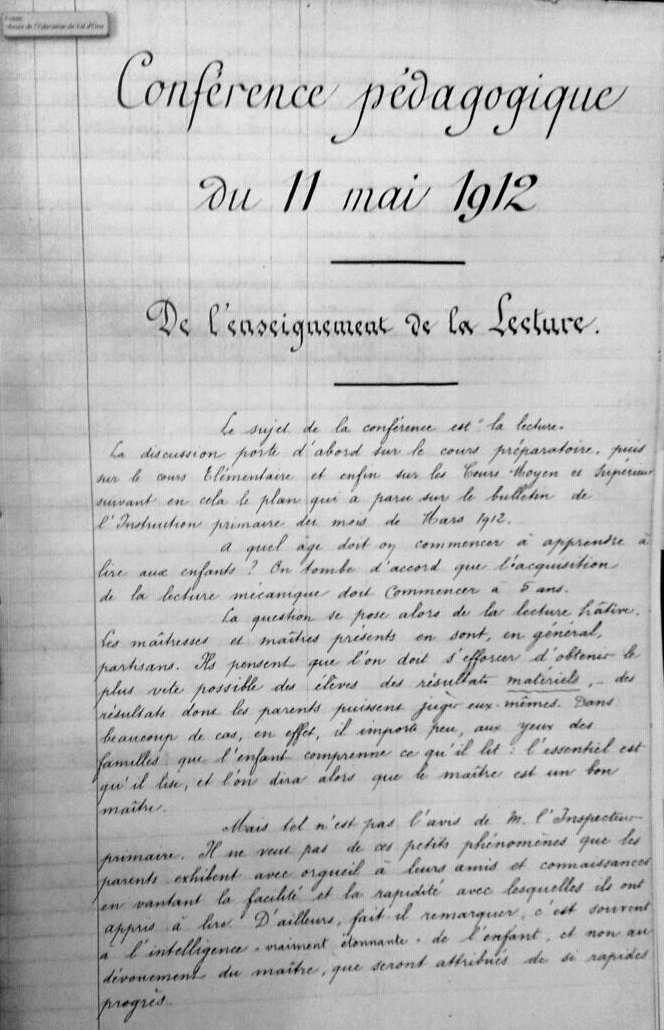
\includegraphics[width=0.6\textwidth]{conf01.png}\\
			    \caption{Retranscription d'une conférence pédagogique de l'école normale de St Germain en Laye de mai 1912. Fond du musée de l'éducation du Val d'Oise.}
			    \label{fig. 4}
			  \end{figure}
			  L'arrêté du 18 janvier 1887 ne dit pas autre chose :
			\begin{quote}
			 \emph{II - l'étude critique des méthodes d'enseignement et des moyens de discipline et d'éducation n'est pas chose nouvelle. Les programmes antérieurs attribuaient au directeur de l'école normale la direction de ces travaux; mais ils prennent, dans la répartition actuelle, une importance inaccoutumée : ils coïncident avec les expériences que les élèves maîtres font aux écoles d'application, tandis qu'autrefois ces expériences précédaient de deux années d'études des méthodes et des procédés scolaires. La conférence pédagogique - trop souvent supprimée jadis - est restaurée, son objet est mieux défini, elle porte sur un ensemble de questions déterminées (leçons faites à des enfants, corrections de devoirs, critiques d'une méthode, d'un manuel de classe, etc.); enfin, obligatoire pour les directeurs des écoles d'application, elle réunit tout le personnel enseignant de l'école normale et devient un exercice d'une valeur capitale, pour où s'élabore et s'affirme l'unité pédagogique de l'école.}
			\end{quote}
			Cet exercice sera constamment réaffirmé, ainsi lors du débat sur le budget de l'instruction publique de 1905 elle réapparait : \emph{"examen critique des méthodes d'enseignement et des moyens d'éducation, examen qui se fait surtout dans les cours et conférences de pédagogie. (...) C'est un avantage aussi, au point de vue de la science pédagogique, si ce n'est au point de vue de la pratique même, de faire ces adaptations en l'absence des enfants : le professeur peut corriger sur le champ la leçon faite, au besoin l'interrompre, la refaire; il peut discuter sur le vif les idées choisies, les procédés employés etc.} M. L. a lui même donné des conférences pédagogiques à l'IUFM ainsi qu'il le déclare : \emph{Je suis intervenu à l'IUFM, il m'est même arrivé de donner une ou deux, dites, conférences pédagogiques}, et nous pouvons encore trouver sur internet des références à des conférences pédagogiques données en IUFM ou au CRDP comme à Rouen\footnote{http://www.cndp.fr/crdp-rouen/index.php/conferences-pedagogiques-20122013}
			Cet exercice n'a toutefois pas, à ce qu'il nous semble, la portée théorique et réflexive du mémoire professionnel instauré lors de la création des IUFM.
			\subsection{Le passage à l'écrit}
			

\part{Ecart entre la volonté des prescripteurs et le travail réel des étudiants}

\section{Pédagogie ou morale, les hussards noirs de la république}

			\subsection{Dissocier morale et pédagogie ?}
			\subsection{Confronter le discours au réel}
			\subsection{enseigner ou éduquer à la morale ?}

\section{Sous les cours, le concours}

			\subsection{Les réformes de 1905 et 1920}
			\subsection{De l'école normale à l'IUFM}
			\subsection{Le CRPE à l'ère de l'IUFM}
			
\section{L'utilité de la formation en question ou devenir enseignant sur le tas}

			\subsection{Forme-t-on à devenir enseignant ?}
			\subsection{Apprendre un métier ou apprendre à avoir un concours ?}
			\subsection{De l'auxillaire au contractuel : le face à face avec la classe}


\part{L'injonction réflexive est-elle opérante pour la formation initiale (et continue ?) des IUFM/ESPE}

\section{Le paradigme de la tête bien faite}
lorem ipsum
			\subsection{Montaigne, Dewey, Schön}
			\subsection{Perrenoud}
			\subsection{•}


\section{La place du concours}

			\subsection{Le concours et le certificat d'études}
			\subsection{Le concours et le baccalauréat}
			\subsection{Le concours et le Master}
			
\section{Du praticien-réflexif au praticien-chercheur}

			\subsection{L'intérêt de la recherche pédagogique pour la pratique}
			\subsection{Le paradigme de la recherche action}
			\subsection{De la recherche en pédagogie à la pédagogie par la recherche}



\part*{Conclusion}
Pour conclure,


\part*{Annexes}
\label{annexe1}

\nocite{*}
\bibliographystyle{apacite}
\bibliography{histoire}

\end{document}
